%!TEX root = ../main.tex
\section{Radio Access Technologies and Global Deployment Status}
\label{sec:technologies_and_deployment}

\begin{table*}[!t]
\centering
\caption{Technical Comparison of V2X Radio Access Technologies~\cite{sudirham2023sdn,anwar2019physical}}
\label{tab:rat_comparison}
\small
\begin{tabular}{lcccc}
\toprule
\textbf{Parameter} & \textbf{IEEE 802.11p} & \textbf{IEEE 802.11bd} & \textbf{LTE-V2X} & \textbf{5G NR-V2X} \\
\midrule
Standard Body & IEEE (2010) & IEEE (2022) & 3GPP Rel. 14/15 (2017) & 3GPP Rel. 16+ (2020) \\
Operating Frequency & 5.855--5.925~GHz & 5.9~GHz, 6~GHz & 5.9~GHz, Cellular & 5.9~GHz, sub-6~GHz, mmWave \\
Channel Bandwidth & 10~MHz (opt. 20) & 10, 20~MHz (to 40) & 10, 20~MHz & 10--100~MHz, 400~MHz \\
Peak Data Rate & 3--27~Mbps (default 6) & 54--108~Mbps+ & 26--50~Mbps & Up to 1~Gbps+ \\
End-to-End Latency & $<$10~ms & $<$5~ms & $<$20~ms & $<$1--3~ms \\
Effective Range & 300--500~m & $\sim$1000~m+ & 450--1000~m & $>$1000~m+ \\
Subcarrier Spacing & 156.25~kHz & 156.25, 312.5~kHz & 15~kHz & 15--60~kHz, 120--240~kHz \\
Channel Coding & Convolutional & LDPC & Turbo & LDPC (Data) / Polar (Ctrl) \\
Channel Access & Decentralised & Decentralised & Scheduled / Autonomous & Scheduled / Autonomous \\
Communication Modes & Broadcast & Broadcast & Broadcast & Broadcast, Groupcast, Unicast \\
Target Use Cases & Basic Safety Beacons & High-Speed Safety & Platooning, Safety & URLLC, Cooperative Perception \\
\bottomrule
\end{tabular}
\end{table*}

To enable vehicular cooperation, vehicles require reliable wireless communication links that can handle high mobility, rapid multipath fading, and dynamically changing network topologies.
Currently, two major technology families provide direct vehicular communications: the IEEE 802.11 standard family and the 3GPP Cellular V2X (C-V2X) family.
This section compares both standard families across their physical (PHY) and medium access control (MAC) layers, evaluates spectrum allocation and multi-Radio Access Technology (multi-RAT) coexistence challenges, and analyses commercial deployment status worldwide.

\subsection{IEEE Standards: 802.11p and 802.11bd}
\label{subsec:ieee_standards}

The IEEE standards are based on adapted versions of Wi-Fi technology for direct, decentralised vehicle-to-everything communications.

\subsubsection{IEEE 802.11p (DSRC / ITS-G5)}
Published in 2010, IEEE 802.11p serves as the access layer for Dedicated Short-Range Communications (DSRC) in North America (supported by the IEEE 1609 Wireless Access in Vehicular Environments (WAVE) protocol stack) and for ITS-G5 in Europe (standardised by the European Telecommunications Standards Institute (ETSI) in EN 302 663).
It operates in the dedicated 5.9~GHz Intelligent Transportation Systems (ITS) frequency band.
At the medium access control layer, IEEE 802.11p provides decentralised, ad-hoc communication without requiring a centralised control system or cellular infrastructure.
This decentralised architecture offers low implementation costs and low end-to-end latency under light channel loads, but lacks coordination across transmitting nodes.

While effective in sparse environments, 802.11p exhibits two major technical drawbacks:
\begin{itemize}
    \item \textbf{Channel Congestion in Dense Traffic:} As vehicle density increases, simultaneous uncoordinated safety beacon broadcasts cause frequent packet collisions and severe packet loss~\cite{szalay2023survey}.
    \item \textbf{Doppler Sensitivity at High Mobility:} At vehicular speeds exceeding 90~km/h, rapid Doppler shifts degrade channel estimation, causing throughput and communication performance to drop sharply compared to lower speeds~\cite{sudirham2023sdn}.
\end{itemize}

\subsubsection{IEEE 802.11bd (Next-Generation V2X)}
To overcome these limitations, the IEEE developed 802.11bd as an evolutionary successor to 802.11p.
IEEE 802.11bd introduces key physical-layer advancements to improve vehicular communications~\cite{sudirham2023sdn}:
\begin{itemize}
    \item \textbf{High Doppler Mitigation:} Enhances channel tracking to maintain low error rates and reliable communications in high Doppler scenarios.
    \item \textbf{Dual Carrier Modulation:} Transmits identical information across subcarriers, boosting signal-to-noise ratio and extending communication range at cell edges.
    \item \textbf{Higher Throughput and Lower Latency:} Delivers higher data throughput and lower communication latency compared to 802.11p.
    \item \textbf{Backward Compatibility:} IEEE 802.11bd frames include legacy-compatible preambles, allowing 802.11bd and legacy 802.11p devices to share the same frequency channel safely.
\end{itemize}
Empirical evaluations show that 802.11bd increases the packet reception ratio from 75\% in 802.11p to over 88\% under identical channel conditions~\cite{sudirham2023sdn}.

\subsection{3GPP Cellular V2X: LTE-V2X and 5G NR-V2X}
\label{subsec:cv2x_standards}

Cellular V2X (C-V2X) was standardised by 3GPP to provide two types of communication: direct PC5 sidelink links, which allow nearby vehicles to talk directly to each other without cellular base stations, and long-range Uu network links, which connect vehicles to cellular base stations over long distances.
While cellular networks offer wide coverage, high throughput, and superior scalability, they also require centralised network management and dedicated infrastructure investments~\cite{sudirham2023sdn}.

\subsubsection{LTE-V2X}
Standardised by 3GPP in Releases 14 and 15 (2017), LTE-V2X provides cellular vehicular communications using 10~MHz or 20~MHz channels in the 5.9~GHz ITS band and commercial cellular frequencies.
On the direct PC5 sidelink, LTE-V2X delivers peak data rates between 26~Mbps and 50~Mbps, end-to-end latency below 20~ms, and an effective communication range between 450~m and 1000~m, exceeding the 300~m to 500~m range of legacy 802.11p~\cite{anwar2019physical,sudirham2023sdn}.
It supports two primary communication interfaces:
\begin{itemize}
    \item \textbf{The Uu Interface:} Connects vehicles to cellular base stations for long-range network services and traffic management.
    \item \textbf{The PC5 Interface:} Enables direct vehicle-to-vehicle (V2V) and vehicle-to-infrastructure (V2I) communication without using base stations.
\end{itemize}

For direct PC5 communication, 3GPP defines two radio resource allocation modes:
\begin{itemize}
    \item \textbf{Mode 3 (Scheduled):} Cellular base stations dynamically assign radio channels to vehicles, which requires network coverage.
    \item \textbf{Mode 4 (Autonomous):} Vehicles select radio channels on their own without network coverage.
    Each vehicle senses channel energy over a past observation window, finds unused resources, and reserves them for its regular safety messages.
\end{itemize}
Mode~4 reliably supports regular safety messages in dense traffic, but packet collisions increase when vehicles suddenly send emergency warnings at the same time~\cite{gyawali2020challenges}.

\subsubsection{5G NR-V2X}
To support advanced autonomous driving services—such as cooperative perception, platooning, and remote driving—3GPP standardised 5G New Radio V2X (NR-V2X) in Release 16 (2020).
Physical layer evaluations show that NR-V2X achieves peak data rates exceeding 1~Gbps and transmission latency between 1~ms and 3~ms, substantially outperforming both LTE-V2X and IEEE 802.11bd~\cite{anwar2019physical,sudirham2023sdn}:
\begin{itemize}
    \item \textbf{Wide Bandwidth and Flexible Spectrum:} Supports channels from 10~MHz up to 100~MHz in sub-6~GHz (FR1) and up to 400~MHz in millimeter-wave (FR2) bands, enabling effective ranges exceeding 1000~m.
    \item \textbf{Flexible Subcarrier Spacing:} Supports configurable subcarrier spacing from 15~kHz to 240~kHz to shorten symbol transmission duration and reduce latency.
    \item \textbf{Multiple Transmission Types:} Supports broadcast, groupcast, and unicast communications, whereas LTE-V2X only supports broadcast.
    \item \textbf{Physical Layer Feedback:} Introduces Hybrid Automatic Repeat Request (HARQ) feedback over the physical sidelink feedback channel, achieving packet reliability above 99.999\%.
    \item \textbf{Enhanced Sidelink Modes:} Introduces Mode~1 (scheduled by base stations) and Mode~2 (autonomous distributed channel selection by vehicles).
\end{itemize}

\subsection{Spectrum Allocation and Multi-RAT Coexistence}
\label{subsec:spectrum_coexistence}

Direct vehicular communication operates within the shared 5.9~GHz ITS band.
However, spectrum scarcity and competing technological ecosystems present major operational challenges.
Because neither standard family alone satisfies all communication requirements across varying traffic densities, multi-RAT architectures have been proposed, as illustrated in Fig.~\ref{fig:multi_rat_arch}.
These hybrid architectures leverage 802.11p for sporadic, low-overhead direct warnings while relying on C-V2X for dense vehicular traffic~\cite{szalay2023survey}.

\begin{figure}[!t]
\centering
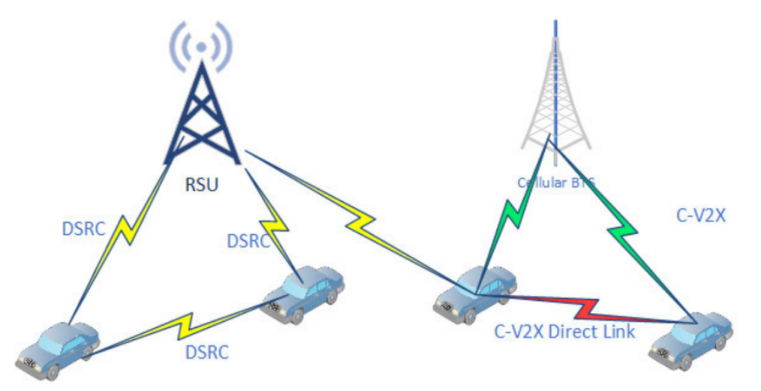
\includegraphics[width=0.88\columnwidth]{figures/rq1/rq1_multi_rat_architecture.png}
\caption{Multi-RAT architecture showing direct DSRC links alongside C-V2X direct sidelink and cellular base station connections~\cite{sudirham2023sdn}.}
\label{fig:multi_rat_arch}
\end{figure}

When both standard families operate in the same 5.9~GHz band without coordination, severe cross-technology interference occurs because nodes cannot detect transmissions across different protocols~\cite{sudirham2023sdn}.
To resolve this coexistence challenge, two primary mechanisms have been developed:
\begin{itemize}
    \item \textbf{Fixed Preamble Insertion:} Inserting fixed preambles into transmissions allows 802.11p and LTE-V2X devices to detect each other's channel occupancy, successfully reducing cross-technology packet collisions in dense traffic~\cite{sudirham2023sdn}.
    \item \textbf{Dynamic RAT Selection and Clustering:} Vehicles form local clusters and dynamically switch between DSRC and C-V2X based on network performance, minimising unnecessary handovers and improving Quality of Service (QoS)~\cite{sudirham2023sdn}.
\end{itemize}

\subsection{Worldwide Commercial Deployment Status}
\label{subsec:deployments}

\begin{figure*}[!t]
\centering
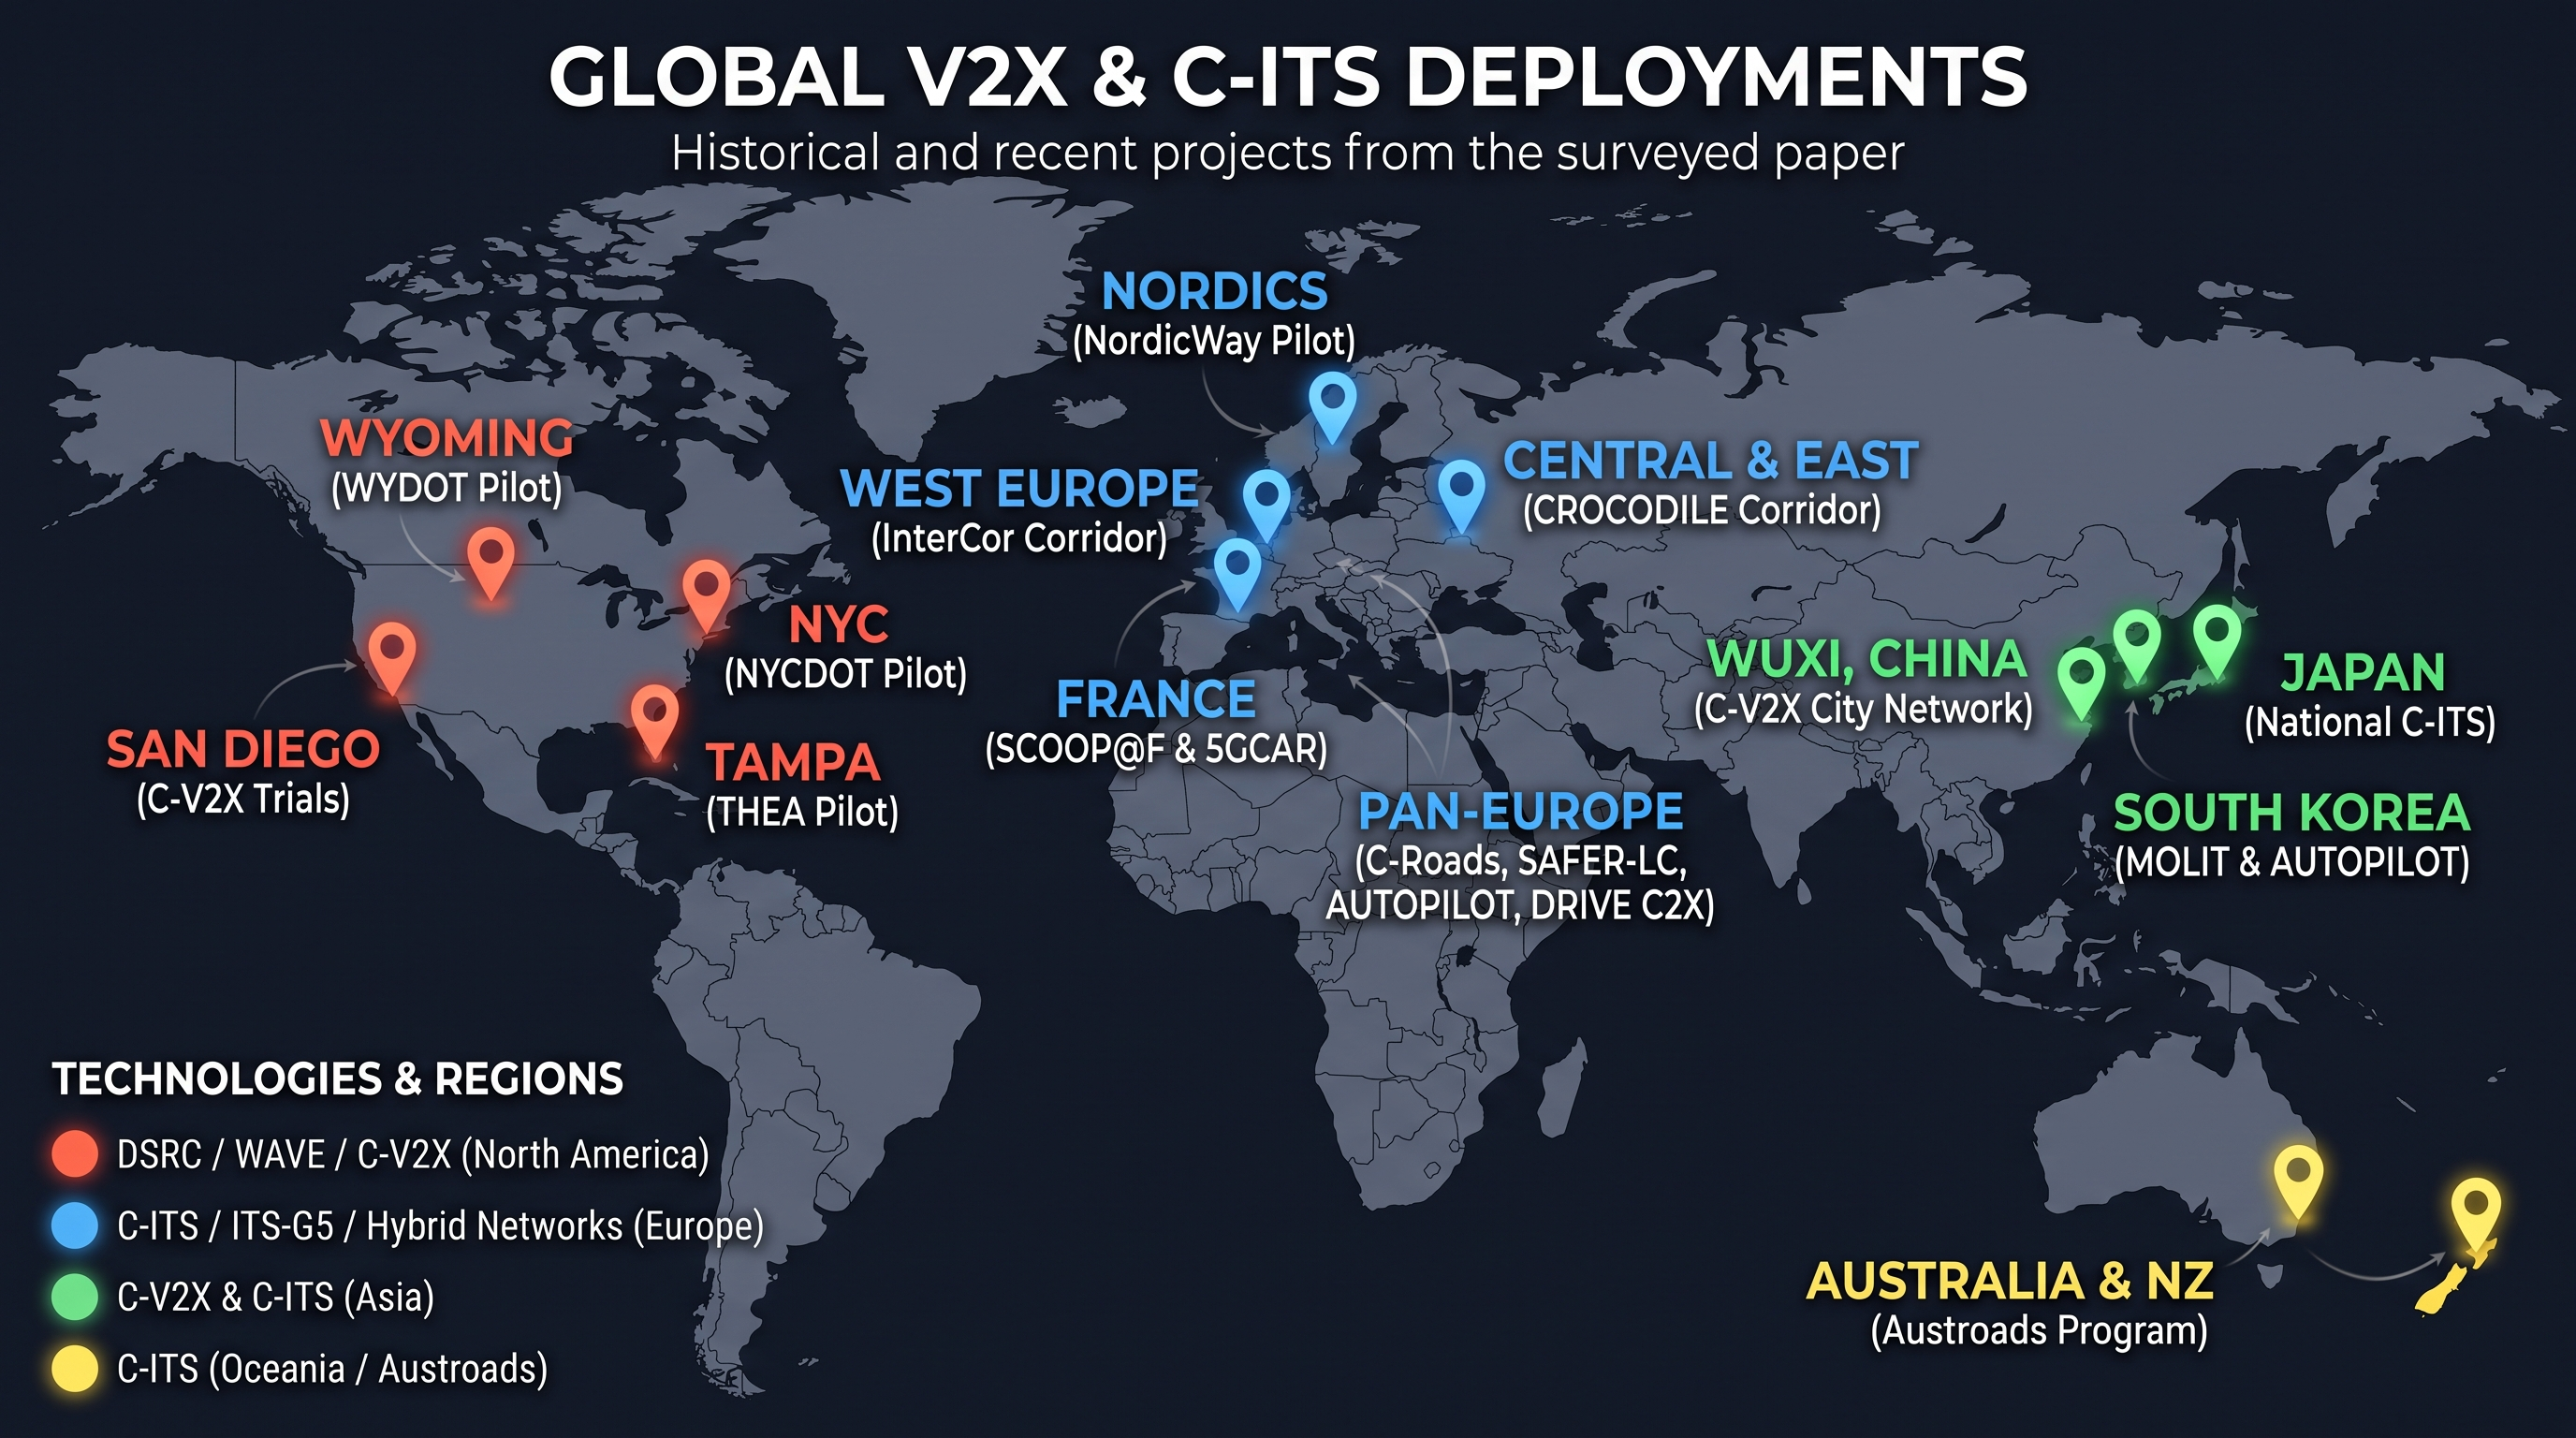
\includegraphics[width=0.88\textwidth]{figures/rq1/rq1_global_v2x_cits_deployments.png}
\caption{Global V2X and C-ITS deployments and pilot projects across North America, Europe, Asia, and Oceania~\cite{szalay2023survey}.}
\label{fig:global_deployments}
\end{figure*}

The commercial deployment of V2X communication technologies varies across different regions due to differing regulatory policies and industry backing, as surveyed by Szalay et al.~\cite{szalay2023survey} and illustrated in Fig.~\ref{fig:global_deployments}.

\subsubsection{United States}
The United States initially pioneered vehicular networking using DSRC.
The U.S. Department of Transportation funded three major connected vehicle pilots in 2015:
\begin{itemize}
    \item \textbf{New York City:} Deployed 353 RSUs and 8,000 equipped vehicles to improve pedestrian safety in high-density urban corridors.
    \item \textbf{Tampa:} Deployed 47 RSUs and over 1,000 equipped cars and buses to reduce morning rush-hour congestion and transit vehicle delays.
    \item \textbf{Wyoming:} Deployed 75 RSUs and 400 commercial trucks along 400 miles of Interstate 80 to reduce winter weather collisions and truck blow-over incidents.
\end{itemize}
Following the 2017 San Diego connected car trials conducted by Qualcomm, Ford, and AT\&T, regulatory decisions redirected American deployment decisively toward C-V2X within the 5.9~GHz band.

\subsubsection{Europe}
Europe has adopted a technology-neutral, hybrid approach under the Cooperative Intelligent Transport Systems (C-ITS) framework, combining ITS-G5 for direct safety-critical messages at intersections with cellular networks for wide-area alerts using standardised ETSI Cooperative Awareness Messages (CAM) and Decentralised Environmental Notification Messages (DENM).
This framework has been validated through major multinational pilots:
\begin{itemize}
    \item \textbf{C-Roads Platform:} Deployed cross-border interoperable Day-1 services (such as hazardous location and slow vehicle alerts) across 16 countries and 43 cities via RSUs and on-board units using the Advanced Message Queuing Protocol.
    \item \textbf{Cross-Border and National Pilots:} The CROCODILE project linked road networks across 13 Central and Eastern European countries for data collection, while France deployed the SCOOP@F pilot connecting 3,000 vehicles over 2,000~km of road.
    The DRIVE C2X project established seven national test sites proving that cooperative speed limit signage reduces road casualties~\cite{szalay2023survey}, while NordicWay tested cellular hazard warning services across Scandinavia.
    \item \textbf{5G Testbeds:} The European 5GCAR project demonstrated 5G testbeds in France for lane-merge coordination and pedestrian protection.
\end{itemize}

\subsubsection{China}
China has adopted a unified national policy centred exclusively on C-V2X.
The Chinese government established dedicated frequency allocations in the 5.9~GHz band and released national standards for vehicular message sets.
Large-scale city deployments include the Wuxi Internet of Vehicles project covering hundreds of urban intersections, alongside national demonstration test zones in Shanghai, Beijing, and Guangzhou.
Major Chinese automobile manufacturers are actively releasing production vehicles equipped with factory-installed C-V2X modules.

\subsubsection{Asia-Pacific and Oceania}
Japan deployed early cooperative systems across its national highway system, and is currently testing C-V2X alongside 5G deployments.
South Korea conducted nationwide highway C-ITS pilots led by the Ministry of Land, Infrastructure, and Transport, testing both LTE-V2X and 802.11p.
Australia and New Zealand developed the Austroads connected vehicle program, evaluating both technologies across major freight routes.
